%%%%%%%%%%%%%%%%%%%%%%%%%%%%%%%%%%%%%%%%%
% Short Sectioned Assignment
% LaTeX Template
% Version 1.0 (5/5/12)
%
% This template has been downloaded from:
% http://www.LaTeXTemplates.com
%
% Original author:
% Frits Wenneker (http://www.howtotex.com)
%
% License:
% CC BY-NC-SA 3.0 (http://creativecommons.org/licenses/by-nc-sa/3.0/)
%
%%%%%%%%%%%%%%%%%%%%%%%%%%%%%%%%%%%%%%%%%

%----------------------------------------------------------------------------------------
%	PACKAGES AND OTHER DOCUMENT CONFIGURATIONS
%----------------------------------------------------------------------------------------

\documentclass[paper=a4, fontsize=11pt]{scrartcl} % A4 paper and 11pt font size

\usepackage[T1]{fontenc} % Use 8-bit encoding that has 256 glyphs
%\usepackage{fourier} % Use the Adobe Utopia font for the document - comment this line to return to the LaTeX default
\usepackage[english]{babel} % English language/hyphenation
\usepackage{amsmath,amsfonts,amsthm} % Math packages
\usepackage{mathtools} %More math! (For dscases)
\usepackage{hyperref} %HTML package
\usepackage{pgfplots} %Makes plots in LaTeX
\usepackage{tikz} %Also tikz?
\usepackage{bbm} %Blackboard bold 1
\usepgfplotslibrary{fillbetween}%Let's me fill between named plots
\usepackage{graphicx} %import pics
\graphicspath{ {Python_figs/} }
\DeclareGraphicsExtensions{.pdf,.png,.jpg}
\usepackage{sectsty} % Allows customizing section commands
\allsectionsfont{ \normalfont\scshape} % Make all sections the default font and small caps


\renewcommand{\thesubsection}{\alph{subsection}} %Make subsections start with letters

\usepackage{fancyhdr} % Custom headers and footers
\pagestyle{fancyplain} % Makes all pages in the document conform to the custom headers and footers
\fancyhead{} % No page header - if you want one, create it in the same way as the footers below
\fancyfoot[L]{} % Empty left footer
\fancyfoot[C]{} % Empty center footer
\fancyfoot[R]{\thepage} % Page numbering for right footer
\renewcommand{\headrulewidth}{0pt} % Remove header underlines
\renewcommand{\footrulewidth}{0pt} % Remove footer underlines
\setlength{\headheight}{13.6pt} % Customize the height of the header

\numberwithin{equation}{section} % Number equations within sections (i.e. 1.1, 1.2, 2.1, 2.2 instead of 1, 2, 3, 4)
\numberwithin{figure}{section} % Number figures within sections (i.e. 1.1, 1.2, 2.1, 2.2 instead of 1, 2, 3, 4)
\numberwithin{table}{section} % Number tables within sections (i.e. 1.1, 1.2, 2.1, 2.2 instead of 1, 2, 3, 4)

\setlength\parindent{0pt} % Removes all indentation from paragraphs - comment this line for an assignment with lots of text

%----------------------------------------------------------------------------------------
%	TITLE SECTION
%----------------------------------------------------------------------------------------

\newcommand{\horrule}[1]{\rule{\linewidth}{#1}} % Create horizontal rule command with 1 argument of height

\title{	Assignment 6}

\author{Benjamin Jakubowski} % Your name

\date{\normalsize\today} % Today's date or a custom date

\begin{document}

\maketitle % Print the title

%----------------------------------------------------------------------------------------
%	PROBLEM 1
%----------------------------------------------------------------------------------------

\section{Uniform distribution}

\subsection{Possible values of $u$}

Let $X_1, X_2, ..., X_n \sim U(0,u)$. Then, given a realization $x_1, x_2, ..., x_n$, the possible values of the parameter u are
\[u \in [x_{max}, \infty)\]
where $x_{max} = \textrm{max} \{x_1, x_2, ..., x_n\}$.

\subsection{Maximum-likelihood estimator $\hat{U}_{ML}$}

We now find the maximum-likelihood estimator $\hat{U}_{ML}$. First, the likelihood function is defined as follows: for $u \in [x_{max}, \infty)$,
\begin{align*}
\mathcal{L}_{\vec{x}} (u) &= \prod_{i = 1}^{n} P_{X_i}(x_i, u) \\
   &= \prod_{i = 1}^{n} \left(\frac{1}{u-0}\right) = \prod_{i=1}^{n} \left(\frac{1}{u}\right) \\
   &= \left(\frac{1}{u}\right)^n
\end{align*}
And, for $u \in (-\infty, x_{max}), \mathcal{L}_{\vec{x}}(u) = 0$.

Now note
\[\mathcal{L}_{\vec{x}}' (u) = (-n) \frac{1}{u}^{n+1} < 0\]
for all $u \in [x_{max}, \infty)$, so $\mathcal{L}_{\vec{x}}$ is monotonically decreasing on this interval. Therefore  $\mathcal{L}_{\vec{x}}(u)$ is maximized by $\hat{U}_{ML} = x_{max}$.

\subsection{PDF of $\hat{U}_{ML}$}
We want to find the PDF of $\hat{U}_{ML} = x_{max}$. We'll first find the CDF, then differentiate to find the PDF.
\begin{align*}
F_{\hat{U}_{ML}}(x) &= P(\hat{U}_{ML} < x) \\
   &= P(x_{max} < x) \\
   &= P\left( \cap_{i = 1}^{n} \left(x_i < x \right)\right) \\
   &= \prod_{i = 1}^{n} P(x_i < x) = \prod_{i = 1} ^{n} \left( \frac{x-0}{u-0}\right) \qquad{} \textrm{ (since the $X_i$ are IID)} \\
   &= \left(\frac{x}{u}\right)^n \\
   &= \left(\frac{1}{u}\right)^n x^n
\end{align*}

So
\[f_{\hat{U}_{ML}}(x) = \frac{\textrm{d}}{\textrm{d}x} F_{\hat{U}_{ML}}(x) = n \left(\frac{1}{u}\right)^n x^{n-1}\]

\subsection{$\hat{U}_{ML}$ is biased}
We now show $\hat{U}_{ML}$ is biased:
\begin{align*}
E(\hat{U}_{ML}) &= \int_0^u x \cdot n \left(\frac{1}{u}\right)^n x^{n-1} \textrm{d}x \\
   &=n \left(\frac{1}{u}\right)^n \int_0^u x^{n} \textrm{d}x \\
   &=n \left(\frac{1}{u}\right)^n \left[ \frac{1}{n+1} x^{n+1}\right]_{x = 0}^{x = u} \\
   &=n \left(\frac{1}{u}\right)^n  \frac{1}{n+1} u^{n+1} \\
   &=\frac{n}{n+1} \cdot u
\end{align*}

Since $E(\hat{U}_{ML}) = \frac{n}{n+1} \cdot u \neq u$, $\hat{U}_{ML}$ is biased.

\subsection{$\hat{U}_{ML}$ converges to u in probability}
We now show $\hat{U}_{ML}$ converges in probability to $u$. Let $\epsilon>0$ be given. Then
\begin{align*}
P\left(\left|\hat{U}_{ML} - u \right| > \epsilon \right) &= 1- P(-\epsilon \leq \hat{U}_{ML} - u \leq \epsilon) \\
   &= 1 - P(u-\epsilon \leq \hat{U}_{ML} \leq u + \epsilon) \\
   &= 1 - \left( P(u-\epsilon \leq \hat{U}_{ML} \leq u) + P(u < \hat{U}_{ML} \leq u + \epsilon) \right)
\end{align*}

But, since $\hat{U}_{ML} = x_{max} \leq u$ we know $P( u < \hat{U}_{ML} \leq u + \epsilon) = 0$. Thus,
\[1 - \left( P(u-\epsilon \leq \hat{U}_{ML} \leq u) + P(u < \hat{U}_{ML} \leq u + \epsilon) \right) = 1 - P(u - \epsilon \leq \hat{U}_{ML} \leq u)\]
Then,
\begin{align*}
1 - P(u - \epsilon \leq \hat{U}_{ML} \leq u) &= 1 - P(u-\epsilon \leq x_{max} \leq u)\\
   &= 1 - \left( 1- P(x_{max} < u - \epsilon) \right)\\
   &= P(x_{max} < u - \epsilon)\\
   &= P\left(\cap_{i = 1}^n (x_i < u - \epsilon)\right)\\
   &= \prod_{i = 1}^n P(x_i < u - \epsilon)\\
   &= \prod_{i = 1}^n \frac{u-\epsilon}{u}\\
   &= \left(\frac{u-\epsilon}{u}\right)^n
\end{align*}

So, to recap: we have shown (given $\epsilon > 0 $),
\[P\left(\left|\hat{U}_{ML} - u \right| > \epsilon \right) = \left(\frac{u-\epsilon}{u}\right)^n\]

Therefore, 
\[\lim_{n \to \infty} P\left(\left|\hat{U}_{ML} - u \right| > \epsilon \right) = \lim_{n \to \infty} \left(\frac{u-\epsilon}{u}\right)^n = 0\]

So $\hat{U}_{ML}$ converges in probability to $u$.

%----------------------------------------------------------------------------------------
%	PROBLEM 2
%----------------------------------------------------------------------------------------

\section{Half life}

\subsection{Parameter of exponential distribution modeling nuclear decay}

Let $h_l$ be the half-life of an element with decay wait time modeled by $T \sim \textrm{Exp}(\lambda)$.
Then
\begin{align*}
P(T < h_l) &= 1/2 \\
\int_0^{h_l} \lambda e^{- \lambda t} \textrm{d}t &= 1/2 \\
1 - e^{-\lambda h_l} &= 1/2 \\
e^{-\lambda h_l} &= 1/2 \\
-\lambda h_l &= \textrm{ln}(1/2) = - \textrm{ln}(2)\\
\lambda &= \frac{\textrm{ln}(2)}{h_l} \\
\end{align*}
Using this equation, the parameter of the distribution for each isotope is calculated below:

\begin{center}
   \begin{tabular}{ | c | c | }
      \hline
      \textbf{Element (isotope)} & \textbf{Parameter($\lambda$)} \\ \hline
      \qquad{} & \qquad{} \\
      Carbon-10 ($\textrm{C}^{10}$) & $\lambda_{\textrm{C}^{10}} = \frac{\textrm{ln}(2)}{19.29} \approx 0.0359$ \\ 
      \qquad{} & \qquad{} \\ \hline
      \qquad{} & \qquad{} \\
      Carbon-15 ($\textrm{C}^{15}$) & $\lambda_{\textrm{C}^{15}} = \frac{\textrm{ln}(2)}{2.45} \approx 0.283$ \\
      \qquad{} & \qquad{} \\\hline
      \qquad{} & \qquad{} \\
      Seaborgium-266 ($\textrm{Sg}^{266}$) & $\lambda_{\textrm{Sg}^{266}} = \frac{\textrm{ln}(2)}{30} \approx 0.0231$ \\ 
      \qquad{} & \qquad{} \\\hline
   \end{tabular}
\end{center}

\subsection{MLE for exponential $\lambda$}

First we find the general MLE for an exponential $\lambda$. Then we consider the question of restricting the set of possible values, or considering $\lambda \in [0,\infty)$. \\

Let $t_1, t_2, ..., t_n$ be the realization of the IID vector $T_1, T_2, ..., T_n \sim \textrm{Exp}(\lambda)$. Then
\begin{align*}
\mathcal{L}_{\vec{t}} (\lambda) &= \prod_{i = 1}^{n} f_{T_i}(t_i, \lambda) \\
   &= \prod_{i = 1}^{n} \left(\lambda e^{-\lambda t_i}\right) \\
   &= \lambda^n e^{-\lambda \sum_{i=1}^n t_i}
\end{align*}

Now we consider
\begin{align*}
\textrm{log } \mathcal{L}_{\vec{t}} (\lambda) &= \textrm{log} \left[ \lambda^n e^{-\lambda \sum_{i=1}^n t_i} \right] \\
   &= n \cdot \textrm{log}(\lambda) - \lambda  \sum_{i=1}^n t_i
\end{align*}

Then $ \frac{\textrm{d}}{\textrm{d}\lambda} \textrm{log } \mathcal{L}_{\vec{t}} (\lambda) = \frac{n}{\lambda} - \sum_{i=1}^n t_i$. Setting this to zero, we find
\begin{align*}
\frac{n}{\lambda} - \sum_{i=1}^n t_i &= 0 \\
\lambda &= \frac{n}{\sum_{i=1}^n t_i}
\end{align*}

Now, let's confirm this is a maximum:
\[\frac{\textrm{d}^2}{\textrm{d}^2 \lambda} \textrm{log } \mathcal{L}_{\vec{t}} (\lambda) = -n \cdot \lambda^{-2}\]
Since the second derivative is negative for all $n \geq 1, \lambda \in (0, \infty)$, this is indeed a maximum. \\

Now that we've found the general MLE  $\hat{\lambda}$, we consider the question of maximizing over a restricted set versus all non-negative reals. In the context of this problem, it would make more sense to consider only $\lambda \in \{\lambda_{C^{10}}, \lambda_{C^{15}}, \lambda_{Sg^{266}}\}$. Our goal is to identify which of the three isotopes is most likely given the observed decay times. In a Bayesian interpretation, this means our prior $P_\Lambda(\lambda) = 0$ for all $\lambda \notin \{\lambda_{C^{10}}, \lambda_{C^{15}}, \lambda_{Sg^{266}}\}$.

\subsection{Posterior distribution}

First, note our prior distribution is
\[
P_{\Lambda}(\lambda) =
\begin{cases}
   P(\lambda_{C^{10}}) \\
   P(\lambda_{C^{15}}) \\
   P(\lambda_{Sg^{266}})
\end{cases}
\]

The likelihood function is
\[P_{\vec{T} | \Lambda} (\vec{t} | \lambda) = \mathcal{L}_{\vec{t}} (\lambda) = \lambda^n e^{- \lambda \sum_{i=1}^n t_i}\]

So, for $\lambda_I$ (the parameter for a given isotope)

\[P_{\Lambda | \vec{T} } (\lambda_I | \vec{t}) = \frac{P_{\Lambda}(\lambda_I) \cdot {\lambda_I}^n e^{- \lambda_i \sum_{i=1}^n t_i}}{\sum_{\lambda \in \{\lambda_{C^{10}}, \lambda_{C^{15}}, \lambda_{Sg^{266}}\}} \left[ P_\Lambda(\lambda) \cdot \lambda^n e^{- \lambda \sum_{i=1}^n t_i}\right]}\]

\subsection{Point estimate for the parameter}

It does not make sense to use the posterior mean as a point estimate of the parameter. The reason is that we are trying to identify the most likely isotope given the data (and our prior beliefs). The posterior mean would likely be an intermediate value- generally
\[E(\Lambda | \vec{T}) \notin \{\lambda_{C^{10}}, \lambda_{C^{15}}, \lambda_{Sg^{266}}\}\]
Instead, our point estimate should just be
\[\hat{\lambda} = \textrm{max} \left\{ P_{\Lambda | \vec{T}} (\lambda | \vec{t}) \big| \lambda \in \{\lambda_{C^{10}}, \lambda_{C^{15}}, \lambda_{Sg^{266}}\} \right\} \]

Note this estimate is called the maximum a posteriori (MAP) estimate (a pedagogical digression- I didn't know what MAP estimates were until this problem, and as a former teacher I found this a really neat way to learn about them).

\subsection{Plotting the posterior distribution}

To inform discussion, two plots are submitted below (while contrary to instructions, I find it necessary to submit these plots to fully explain the results):
\begin{center}
   \begin{tabular}{ c c }
      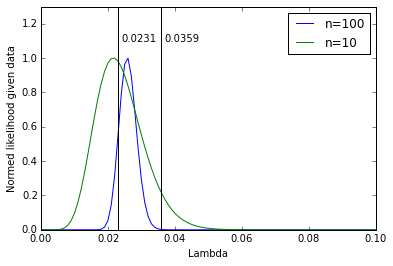
\includegraphics[scale=0.5]{Q2e_fig2} & 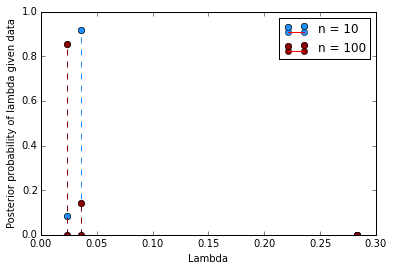
\includegraphics[scale=0.5]{Q2e_fig1}\\
   \end{tabular}
\end{center}

First, consider the left plot (showing the normed likelihood function). The likelihood function for $n = 10$ is less concentrated compared to the likelihood function for $n=100$ (which makes sense, given the MLE converges to $\lambda$ as $n \to \infty$). As such, the likelihood of $\lambda_{C^{10}} = 0.0359$ is much greater when $n=10$ than when $n=100$ (even though both functions have similar modes).\\

Moreover (now considering $n=10$), even though the likelihood of $\lambda_{C^{10}} = 0.0359$ is still lower than the likelihood $\lambda_{Sg^{266}} = 0.0231$, the dramatic difference in priors (recall $P_{\Lambda}(\lambda_{C^{10}}) = 0.49$, while $P_{\Lambda}(\lambda_{Sg^{266}}) = 0.01$) means the posterior probability of $\lambda_{C^{10}}$ is much greater.\\

In conclusion, even though the MLE (maximizing over the set $\{\lambda_{C^{10}}, \lambda_{C^{15}}, \lambda_{Sg^{266}}\}$) $\hat{\lambda}_{MLE} = \lambda_{Sg^{266}} $ is the same for $n=10, n=100$, the MAP estimate $\hat{\lambda}_{MP}$ changes with $n$.


%----------------------------------------------------------------------------------------
%	PROBLEM 3
%----------------------------------------------------------------------------------------

\section{Empirical probability mass function}

\subsection{Nonparametric estimator for the PMF of A (age)}

Given we are trying to estimate the distribution of ages in years, a reasonable non-parametric estimator is

\[\hat{P}_A(a) = \frac{1}{n} \sum_{i = 1}^{n} \mathbbm{1}_{x_i = a} \]

where $a$ is an age in years.

\subsection{$\hat{P}_A(a)$ is unbiased}

To show $\hat{P}_A(a)$ is unbiased, we must show $E(\hat{P}_A(a)) = P_A(a)$ for all $a$. Well,
\begin{align*}
E(\hat{P}_A(a)) &= E\left( \frac{1}{n} \sum_{i = 1}^{n} \mathbbm{1}_{x_i = a}\right) \\
   &=  \frac{1}{n} \sum_{i = 1}^{n} E\left(\mathbbm{1}_{x_i = a}\right)
\end{align*}
But, for all $i \in \{1, 2, ..., n\}, E(\mathbbm{1}_{x_i = a}) = P_{X_i}(a)$
Now, assume the $X_i$ are IID, and follow the underlying distribution of the population (i.e. $P_{X_i}(a) = P_A(a)$). Then
\begin{align*}
E(\hat{P}_A(a)) &=  \frac{1}{n} \sum_{i = 1}^{n} E\left(\mathbbm{1}_{x_i = a}\right)\\
   &= \frac{1}{n} \sum_{i = 1}^{n} P_A(a) \\
   &= \frac{1}{n} n P_A(a) \\
   &= P_A(a)
\end{align*}

So $\hat{P}_A(a)$ is unbiased (under the previously articulated assumptions).

\subsection{$\hat{P}_A(a)$ is consistent}

First, recall $\hat{P}_A(a)$ is consistent if $\lim_{n \to \infty} E\left((\hat{P}_A(a) - P_A(a))^2\right) = 0$.
Now note
\begin{align}
E\left((\hat{P}_A(a) - P_A(a))^2\right) &= E\left(\hat{P}_A(a)^2 - 2P_A(a)\hat{P}_A(a) + P_A(a)^2\right) \nonumber \\
   &= E\left(\hat{P}_A(a)^2\right) - 2P_A(a)E\left(\hat{P}_A(a)\right) + P_A(a)^2  \nonumber \\
   &= E\left(\hat{P}_A(a)^2\right) - 2P_A(a)^2 + P_A(a)^2 \qquad{} \textrm{ (since $\hat{P}_A(a)$ is unbiased)}  \nonumber \\
   &= E\left(\hat{P}_A(a)^2\right) - P_A(a)^2 \label{eq:test}
\end{align}

Thus, to determine if $\hat{P}_A(a)$ is consistent, we need to evaluate $E\left(\hat{P}_A(a)^2\right)$.

\begin{align*}
E\left(\hat{P}_A(a)^2\right) &= E\left( \left(  \frac{1}{n} \sum_{i = 1}^{n} \mathbbm{1}_{x_i = a} \right)^2\right) \\
   &= E\left(  \frac{1}{n^2} \sum_{i = 1}^{n}\sum_{j = 1}^{n} \mathbbm{1}_{x_i = a}\mathbbm{1}_{x_j = a} \right)\\
   &= \frac{1}{n^2} \sum_{i = 1}^{n} P_A(a) + \frac{1}{n^2}\sum_{i=1}^{n} \sum_{\substack{j = 1 \\ j \ne i}}^{n}\left(P_A(a)\right)^2\\
   &= \frac{1}{n} P_A(a) + \frac{n-1}{n}P_A(a)^2
\end{align*}

Now, substituting into expression \eqref{eq:test} yields
\begin{align*}
   E(\hat{P}_A(a)^2) - P_A(a)^2 &= \frac{1}{n} P_A(a) + \frac{n-1}{n}P_A(a)^2 - P_A(a)^2 \\
   &=  \frac{1}{n} P_A(a) + \frac{1}{n}P_A(a)^2 \\
   &=  \frac{1}{n} \left(P_A(a) + P_A(a)^2 \right)
\end{align*}

So 
\[\lim_{n \to \infty} E\left(\left(\hat{P}_A(a) - P_A(a)\right)^2\right) = \lim_{n \to \infty} \left(\frac{1}{n} \left(P_A(a) + P_A(a)^2 \right) \right) = 0\]

Thus, $\hat{P}_A(a) \to P_A(a)$ in mean square (and, also, by implication, in probability).

\subsection{Estimator performance at higher granularity}

If we record the age at a higher granularity, we will likely end up with many empty bins (i.e. values of $a\in R_A$ such that $x_i \ne a$ for all $i \in \{1, 2, ..., n\}$. For these $a$, our estimate $\hat{P}_A(a) = 0$ (even though we would want non-zero probability estimates for all reasonable ages). More generally, our estimator is not very robust (in the sense that it won't perform well for small $n$ or at higher granularity).


%----------------------------------------------------------------------------------------
%	PROBLEM 4
%----------------------------------------------------------------------------------------

\section{Call Center}

\subsection{MLE estimator for Poisson $\lambda$}

Let $x_1, x_2, ..., x_n$ be realizations of IID $X_1, X_2, ..., X_n \sim \textrm{Poisson}(\lambda)$. Recall, first, that
\[f_{X_i}(k) = \frac{\lambda^k}{k!} e^{-\lambda}\]
Then
\begin{align*}
\mathcal{L}_{\vec{x}}(\lambda) &= \prod_{i = 1}^n f_{X_i}(x_i, \lambda) \\
   &=\prod_{i = 1}^n \left( \frac{\lambda^{x_i}}{x_i!} e^{-\lambda} \right) \\
   &=\frac{\lambda^{\sum_{i=1}^n x_i}}{\prod_{i=1}^n x_i!} e^{-n \lambda} \\
\end{align*}
So
\[\textrm{log} \mathcal{L}_{\vec{x}}(\lambda) = \textrm{log} (\lambda) \sum_{i=1}^n x_i - n \lambda - \sum_{i=1}^n \textrm{log} (x_i!)\]
Then
\[\frac{\textrm{d}}{\textrm{d}\lambda} \textrm{log} \mathcal{L}_{\vec{x}}(\lambda) = \frac{\sum_{i=1}^n x_i }{\lambda} - n\]\
Setting this equal to zero, we find
\begin{align*}
0 &= \frac{\sum_{i=1}^n x_i }{\lambda} - n \\
\implies \qquad{} \lambda &= \frac{1}{n} \sum_{i=1}^n x_i 
\end{align*}
Again, let's check this is a maximum:
\[ \frac{\textrm{d}^2}{\textrm{d}^2\lambda} \textrm{log} \mathcal{L}_{\vec{x}}(\lambda) = - \sum_{i=1}^n x_i \lambda^{-2} < 0 \]
(since $\lambda \geq 0, x_i \geq 0 \textrm{ for all } i$).
Thus this is indeed a maximum.

\subsection{Comparing parametric and non-parametric estimation}

First, recall our goal was to estimate the distribution of the calls in October using (i) two days of data from the beginning of October, and (ii) data from the entire month of September. Parametric (MLE) and non-parametric estimators were constructed and estimation errors were determined using the $l_1$ norm of the difference in distributions. These errors are presented below:
\begin{center}
   \begin{tabular}{ | c | c | c | }
   \hline
   \textbf{Data} & \textbf{MLE fitting errors} & \textbf{Nonparametric fitting errors} \\ \hline
   2 days & 0.4334 & 0.5185 \\ \hline
   September & 0.5072 & 0.4028 \\ \hline
   \end{tabular}
\end{center}
      
\subsection{Comparing parametric and non-parametric estimation- continued}

Based on these errors, it appears parametric (MLE) estimation performs best for the 2-day data. In contrast, nonparametric estimation performs better for the September data. This suggests that parametric estimation is better when less data is available, while non-parametric estimation is better when more data is available. This assertion is not only supported by the results from this particular modeling problem- it also makes theoretical sense through the lens of bias-variance tradeoff.\\

First, looking at the plotted non-parametric estimated distribution, the 2-day estimate is very noisy. This illustrates that with less data, model variance is higher and dominates the total estimation error. On the other hand, using parametric estimation constrains the model, reducing model variance (though potentially inflating bias). With less data, this reduction in variance results in overall lower error (i.e. it is more significant than any potential increase in bias).\\

Now, consider the estimates constructed using September data. When more data is available, non-parametric estimation outperforms parametric estimation. This is because the parametric estimate may be biased if the underlying process does not truly follow the Poisson distribution. With more data, the reduction in variance achieved through parametric estimation (i.e by constraining our model space) does not outweigh the error cost incurred due to inflated bias.


%----------------------------------------------------------------------------------------
%	PROBLEM 5
%----------------------------------------------------------------------------------------

\section{Method of Moments (MM) estimators}

Note that in all cases, let $x_1, x_2, ..., x_n$ be realizations of $X_1, X_2, ... X_n \sim D(c)$, where the $D$ is the distribution specified in the subproblem, and $c$ is the target parameter.

\subsection{Bernoulli distribution}

First, recall (from the notes) that $\hat{p}_{MLE} = \frac{n_1}{n_1 + n_0}$. Now, $E(X_i) = p$, and $\bar{x}_n = \frac{1}{n} \sum_{i = 1}^{n}x_i$. Thus, setting $\bar{x}_n = E(X_i)$ yields:
\begin{align*}
\hat{p}_{MM} &= \frac{1}{n} \sum_{i = 1}^{n}x_i \\
   &= \frac{n_1}{n_1 + n_0} = \hat{p}_{MLE}
\end{align*}

\subsection{Geometric distribution}

First, we derive the MLE for a geometric distribution. Recall $f_{X_i}(k) = (1-p)^{k-1} p$. Thus

\begin{align*}
\mathcal{L}_{\vec{x}} (p) &= \prod_{i = 1}^{n} f_{X_i}(x_i, p) \\
   &= \prod_{i = 1}^{n} \left((1-p)^{x_i-1} p\right) \\
   &= p^n (1-p)^{\sum_{i=1}^n (x_i -1)} \\ 
   &= p^n (1-p)^{\sum_{i=1}^n (x_i) -n} \\ 
\end{align*}

Now we consider
\begin{align*}
\textrm{log } \mathcal{L}_{\vec{x}} (p) &= \textrm{log} \left(p^n (1-p)^{\sum_{i=1}^n (x_i) -n}\right) \\
   &= n \cdot \textrm{log}(p) +\textrm{log}(1-p)\left( \sum_{i=1}^n (x_i) - n \right)
\end{align*}
Then 
\[\frac{\textrm{d}}{\textrm{d}p} \textrm{log } \mathcal{L}_{\vec{x}} (p) = n \frac{1}{p} - \left(\sum_{i=1}^n (x_i) - n\right)\frac{1}{1-p}\]
Setting this to zero, we find
\begin{align*}
n \frac{1}{p} - \left(\sum_{i=1}^n (x_i) - n\right)\frac{1}{1-p} &= 0 \\
\implies \qquad{} \left(\sum_{i=1}^n (x_i) - n\right)\frac{1}{1-p} &= n \frac{1}{p} \\ 
\implies \qquad{} p \left(\sum_{i=1}^n (x_i) - n\right) &= n (1-p) \\ 
\implies \qquad{} p \sum_{i=1}^n x_i &= n \\ 
\implies \qquad{} p &= \frac{n}{ \sum_{i=1}^n x_i} \\ 
\end{align*}

Now, let's confirm this is a maximum:
\[\frac{\textrm{d}^2}{\textrm{d}^2 p} \textrm{log } \mathcal{L}_{\vec{x}} (p) = -n \cdot p^{-2} - \left(\sum_{i=1}^n (x_i) - n\right)(1-p)^{-2}\]
Since the second derivative is negative for all relevant values of $x_i, n,$ and $p$, this is indeed a maximum. \\

Now, $E(X_i) = 1/p$. Thus, setting $\bar{x}_n = E(X_i)$ yields:
\begin{align*}
\frac{1}{\hat{p}_{MM}} &= \frac{1}{n} \sum_{i = 1}^{n}x_i \\
   \implies \qquad{} \hat{p}_{MM} &= \frac{n}{\sum_{i = 1}^{n}x_i} = \hat{p}_{MLE}
\end{align*}


\subsection{Poisson distribution}

First, recall (from problem 4(a)) that $\hat{\lambda}_{MLE} = \frac{1}{n} \sum_{i=1}^n x_i$.

Now, $E(X_i) = \lambda$. Thus, setting $\bar{x}_n = E(X_i)$ yields:
\[\hat{\lambda}_{MM} = \frac{1}{n} \sum_{i=1}^n x_i = \hat{\lambda}_{MLE}\]

\subsection{Exponential distribution}

First, recall (from problem 2(b)) that $\hat{\lambda}_{MLE} =\frac{n}{\sum_{i = 1}^{n}x_i}$.

Now, $E(X_i) = \frac{1}{\lambda}$. Thus, setting $\bar{x}_n = E(X_i)$ yields:
\begin{align*}
\frac{1}{\hat{\lambda}_{MM}} &= \frac{1}{n} \sum_{i = 1}^{n}x_i \\
   \implies \qquad{} \hat{\lambda}_{MM} &= \frac{n}{\sum_{i = 1}^{n}x_i} = \hat{\lambda}_{MLE}
\end{align*}

 %----------------------------------------------------------------------------------------
\end{document}